\chapter{PhytoMFTM - a flexible object-oriented PFT model}


\small {\textbf{This is the work towards the second manuscript, to be submitted to Geoscientific Model Development (GMD)}}


\normalsize
\section{Python ecosystem model package development}
The developments in computational capacities and tools have revolutionized the field of ecology. Where models were first only mathematically solved, soon they could be run on highly specialized computers until today where anybody can code or run a model on their personal computer, smartphone or even a cloud platform. This allows much greater reproducibility and makes sharing model code, results and statistical analysis much easier. Science can greatly benefit from this, even though there are many barriers to completely "Open Science". Open Science refers to transparency at all stages of the scientific process \citep{Hampton2015}.

\begin{figure}
\centering
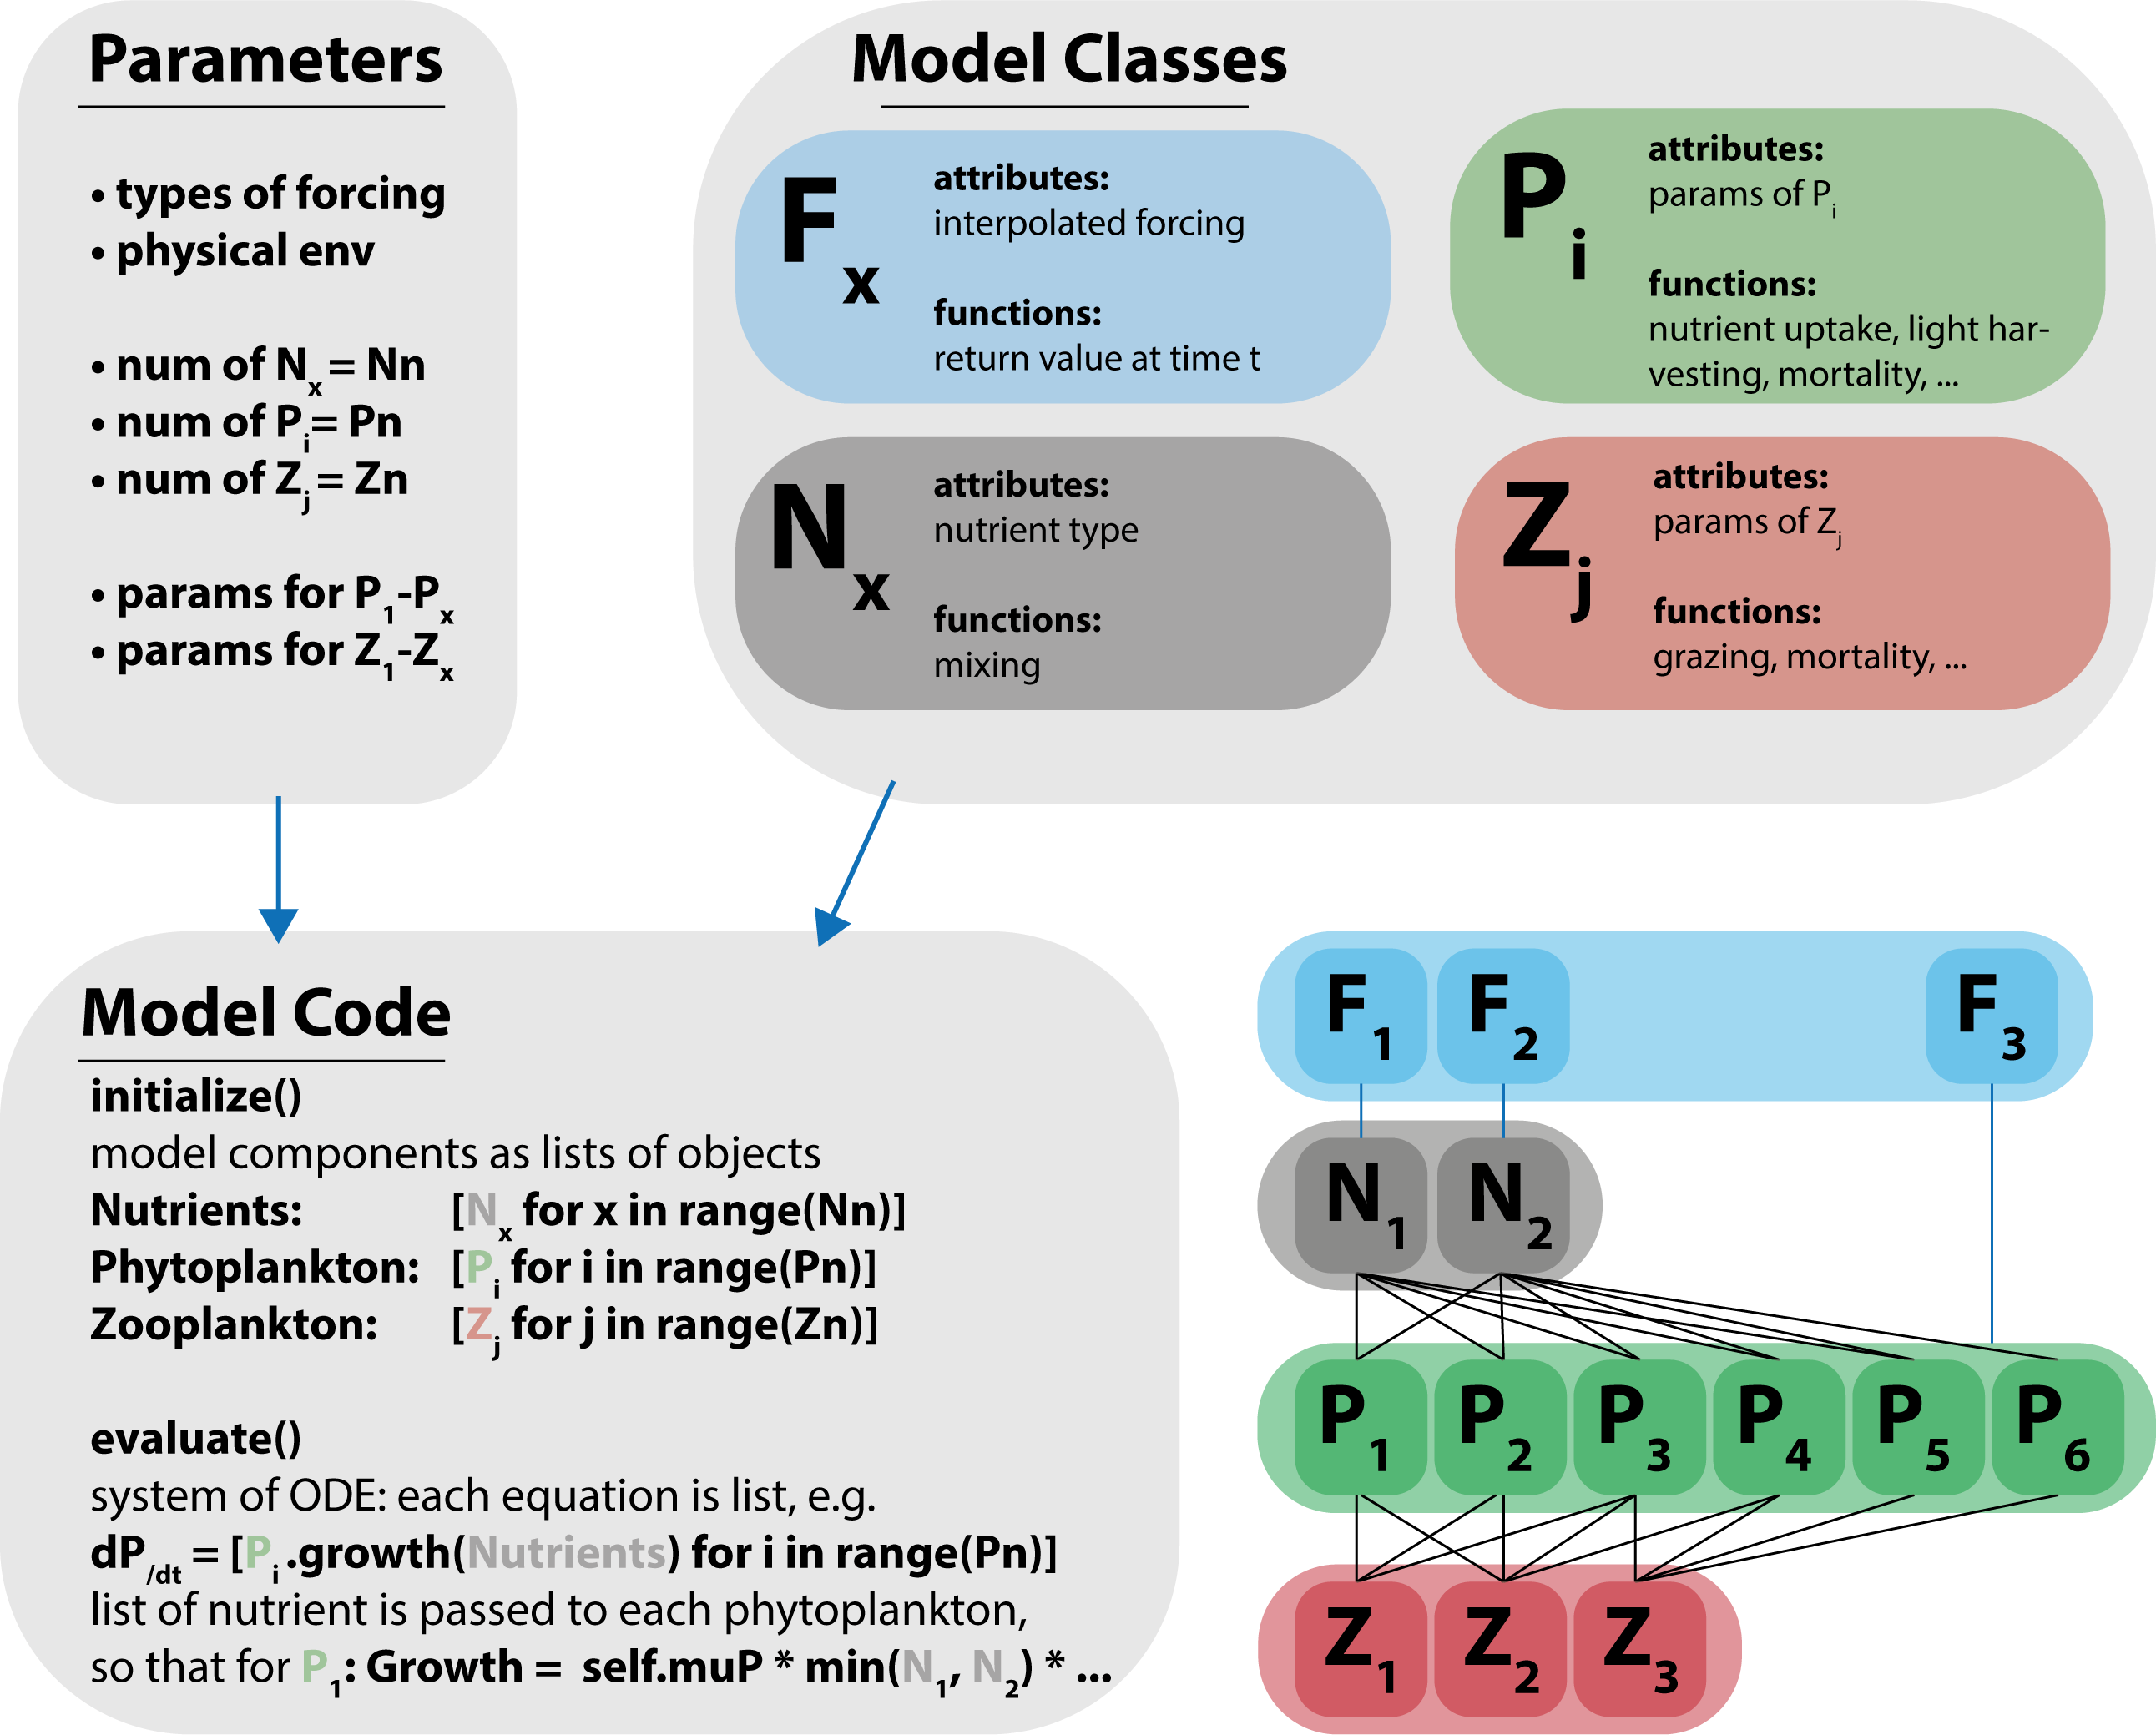
\includegraphics[trim = 0mm 0mm 0mm 0mm, clip, width=1.\linewidth]{./Chp22-Pre2/OOPmodelstructureDraft.png}
\caption[Scheme]{\small {Schematic of code structure for PhytoMFTM model. Square brackets ("[ ]") denote a list object in Python,"for i in range(x)" within brackets creates list of length x of whatever comes before. Model classes are used to store both the parameters associated with each instance, e.g. different nutrient uptake parameters for PFTs and the functions that are used within the ODE. Each equation is also a list structure that calls every instance of the required objects using list comprehensions, so that all interactions are calculated according to the number of model components that were initialized in the parameters.}}
\label{PhytoMFTM}
\end{figure}

Given that code is easily shared, this can be well implemented in ecological modeling research. There are different attempts at unified modeling frameworks, but most researchers still use different tools depending on their experience and computational literacy \citep{Michener2012}. The development of open-source modeling packages is a step in the direction of greater reproducibility and collaboration in ecological research. The modeling community is moving towards open-source tools and in particular the programming language Python is growing in popularity \citep{Lin2012}. The idea to publicly share my model code and develop a well documented Python package to be used by other researchers was inspired by the PhytoSFDM model \citep{Acevedo-Trejos2016}. The PhytoMFTM model structure itself will allow for flexible implementations of different kinds of ecosystem models. 






{\textbf{Object-oriented structure}}

The model code used in the previous section was developed with flexibility in mind. The main reason for building this code was that at the start of the project, I did not know yet how many functional types will have to be implemented. Instead of manually adding a new equation, each equation is implemented as a list of equations (see Figure \ref{PhytoMFTM}). These lists contain the functions to be solved and iterate over a list of all model components. Each model class, like a phytoplankton type for example, contains the parameters assigned to it so that each individual interaction can be called upon as the equation iterates over the contained list. In theory this allows for an arbitrary number of model components, only constrained by computational costs that increase with each instantiated object. The object-oriented code allows for efficient calculation, particularly in relatively simple applications. For a model structure as used in Section 2 a five year run can be calculated in 2.5 seconds. 



